\documentclass[bibtotocnumbered]{article}
\usepackage[english]{babel}

\usepackage[utf8]{inputenc}
\usepackage{amsmath}
\usepackage{titlesec}
\usepackage{xcolor}
\usepackage{sectsty}
\usepackage[T1]{fontenc}
\usepackage{XCharter}
\usepackage{glossaries}
\usepackage{graphicx}
\usepackage[toc,page]{appendix}
\usepackage[
top    = 1in,
bottom =1in,
left   = 1in,
right  = 1in]{geometry}
\usepackage[parfill]{parskip}
\usepackage[utf8]{inputenc}
\usepackage{fancyhdr}
\usepackage[backend=biber, style=authoryear]{biblatex}
\addbibresource{refs.bib}
\usepackage{hyperref}
\setcounter{secnumdepth}{4}

\titleformat{\paragraph}
{\normalfont\normalsize\bfseries}{\theparagraph}{1em}{}
\titlespacing*{\paragraph}
{0pt}{3.25ex plus 1ex minus .2ex}{1.5ex plus .2ex}
\begin{document}
\section{Designs}
\subsection{System Design}
\subsubsection{Class diagrams and mind map}
The developer used a mind map to initially appraise the connection between each musical symbol. This helped break down a piece from a musician's view, and showed what information would be necessary between each symbol's class.

An initial class diagram was drawn from the mind map. This was modified during the course of development testing and research of the initial model. In particular, the developer looked at other sources such as Music21, a toolkit for computer-aided musicology\parencite{Music21}, which helped the developer to examine whether the initial model was missing any classes or attributes. The diagrams described are in the appendices.
\subsection{UI Design}
The User interface for this project is designed with the average musician in mind, and the interfaces that user would normally have used. With this in mind, the designs explained below and shown in Appendix D are inspired by other music applications in common usage.

\subsubsection{Main Display}
\begin{center}
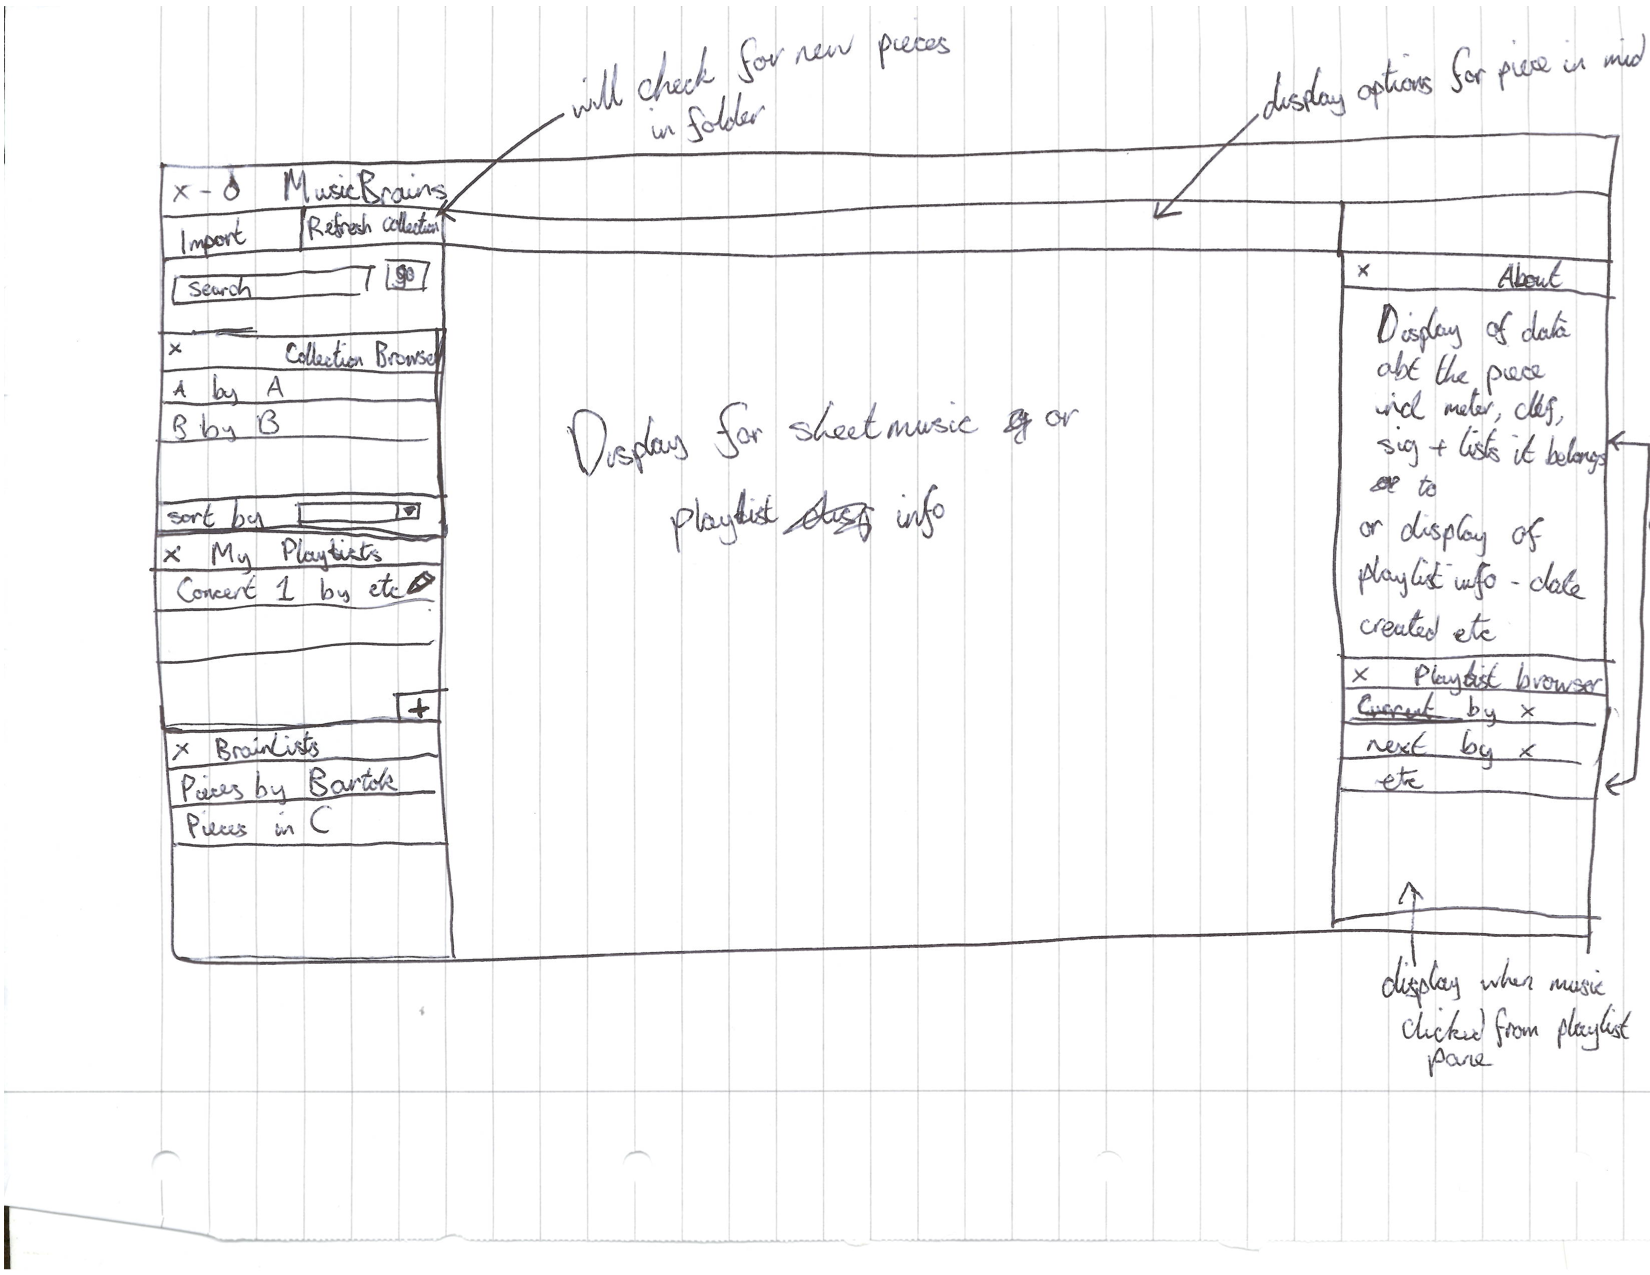
\includegraphics[width=380pt]{main_view.png}
\end{center}

The above image shows the main view of the application. Various panes to the left can be closed using the X button and show different ways the music can be displayed, either as individual units or as playlists. The panes to the right display content based on what is selected for display in the middle, larger window, generally either a playlist or a singular piece of sheet music. Updates to these panes and various pop up boxes associated with different buttons in the display are in the appendices.
\subsubsection{Musician feedback survey}
In order to understand how well this user interface works with a variety of users, a survey was designed which will be given to a selection of musicians, who will feedback on how easy the UI is to use and any updates which should be made to improve it. This feedback session will be performed after the initial sketches are made into a virtual user interface with no back end connected to the buttons. An example survey is provided in the appendices.
\subsection{Test Design}
The developer has chosen to use test driven development. This is an agile software development methodology which utilises the rules that the developer should never write a signle line of code unless there is a failing automated test\parencite{TDD}. This methodology has been chosen as the nature of the notation of music means that meticulous detail must be payed to how and with what symbol every element is notated, and Test Driven Development will ensure that every detail has been validated and proven to work.

The list of tests to date, which are written on an adhoc basis as the developer builds up functionality, are attached in the appendices, along with a description of current testcases used to confirm the functionality works with real world examples of sheet music.
\begin{appendices}
\section{Revised computerised class diagram}
\section{Initial User Interface Design}
\subsection{Main Display}
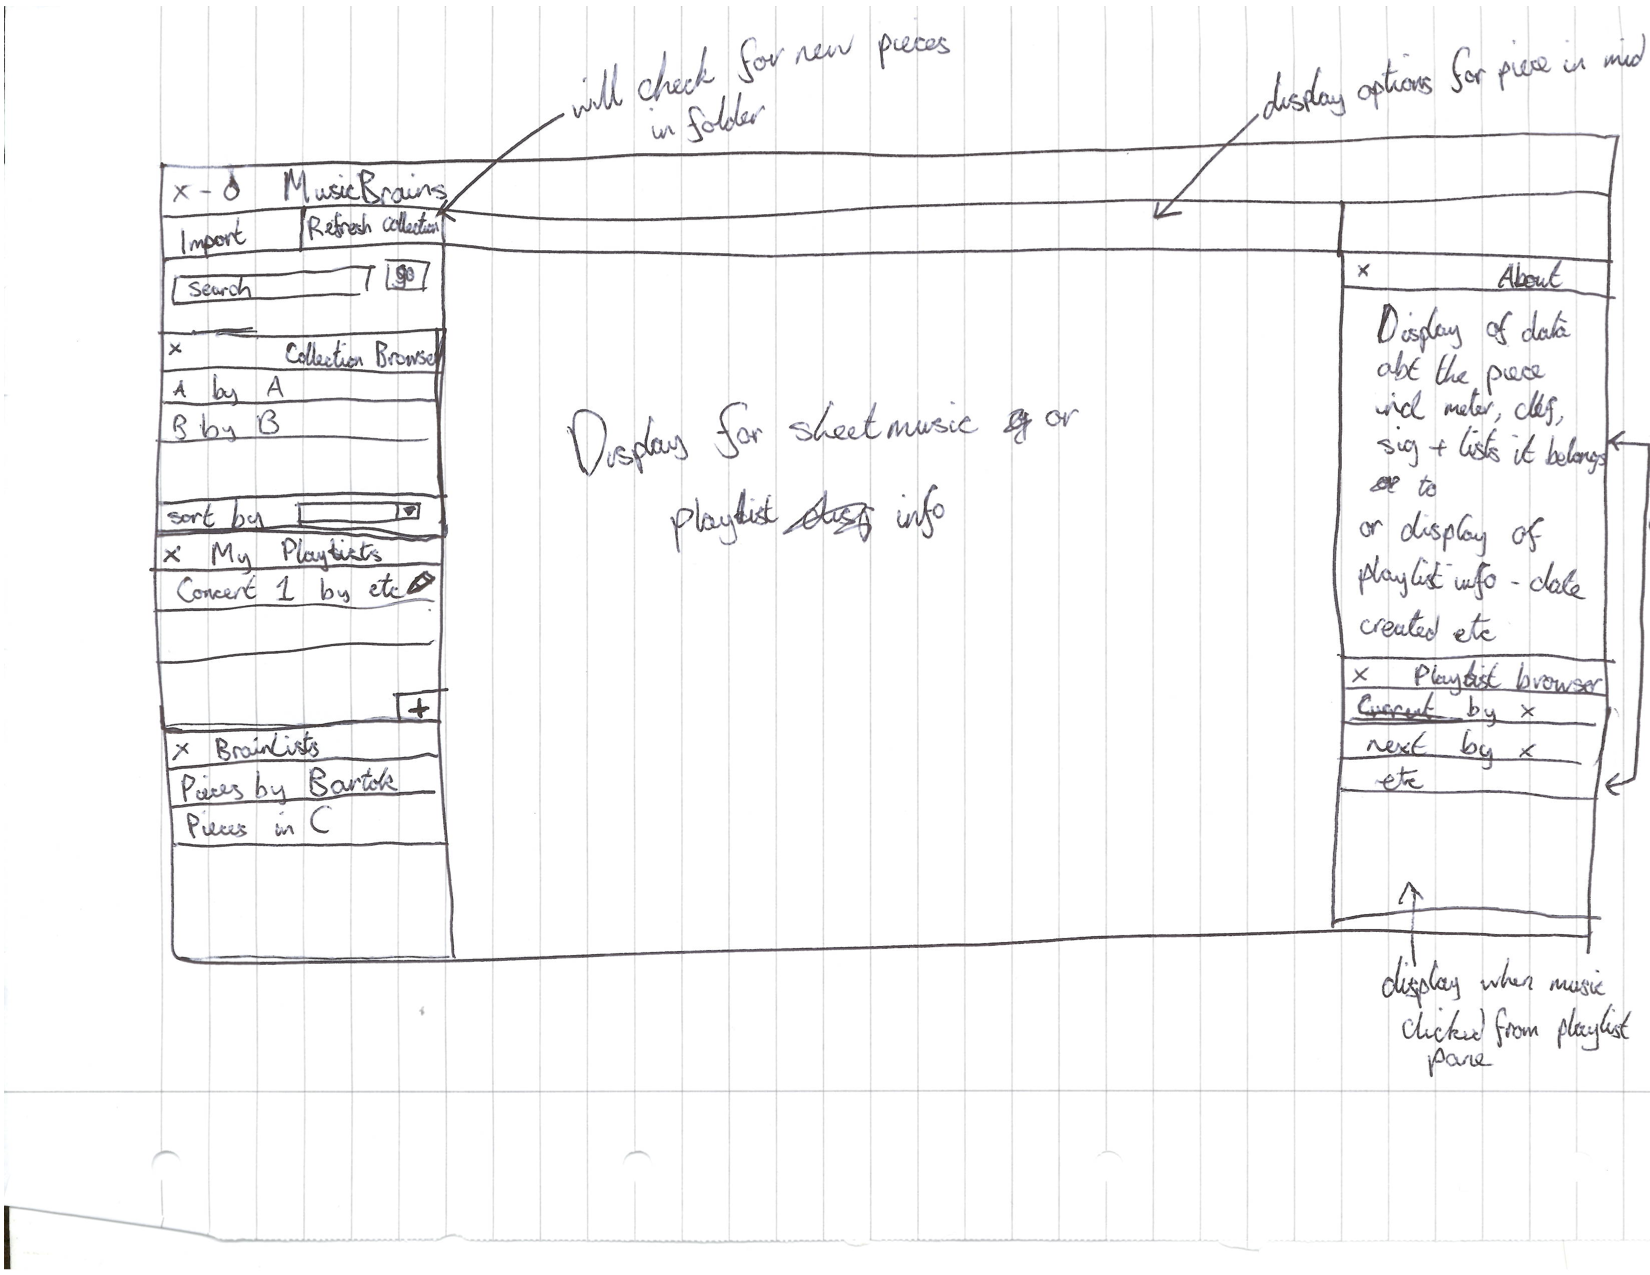
\includegraphics[width=500pt]{main_view.png}
\subsection{Changes to main display when sheet music selected}
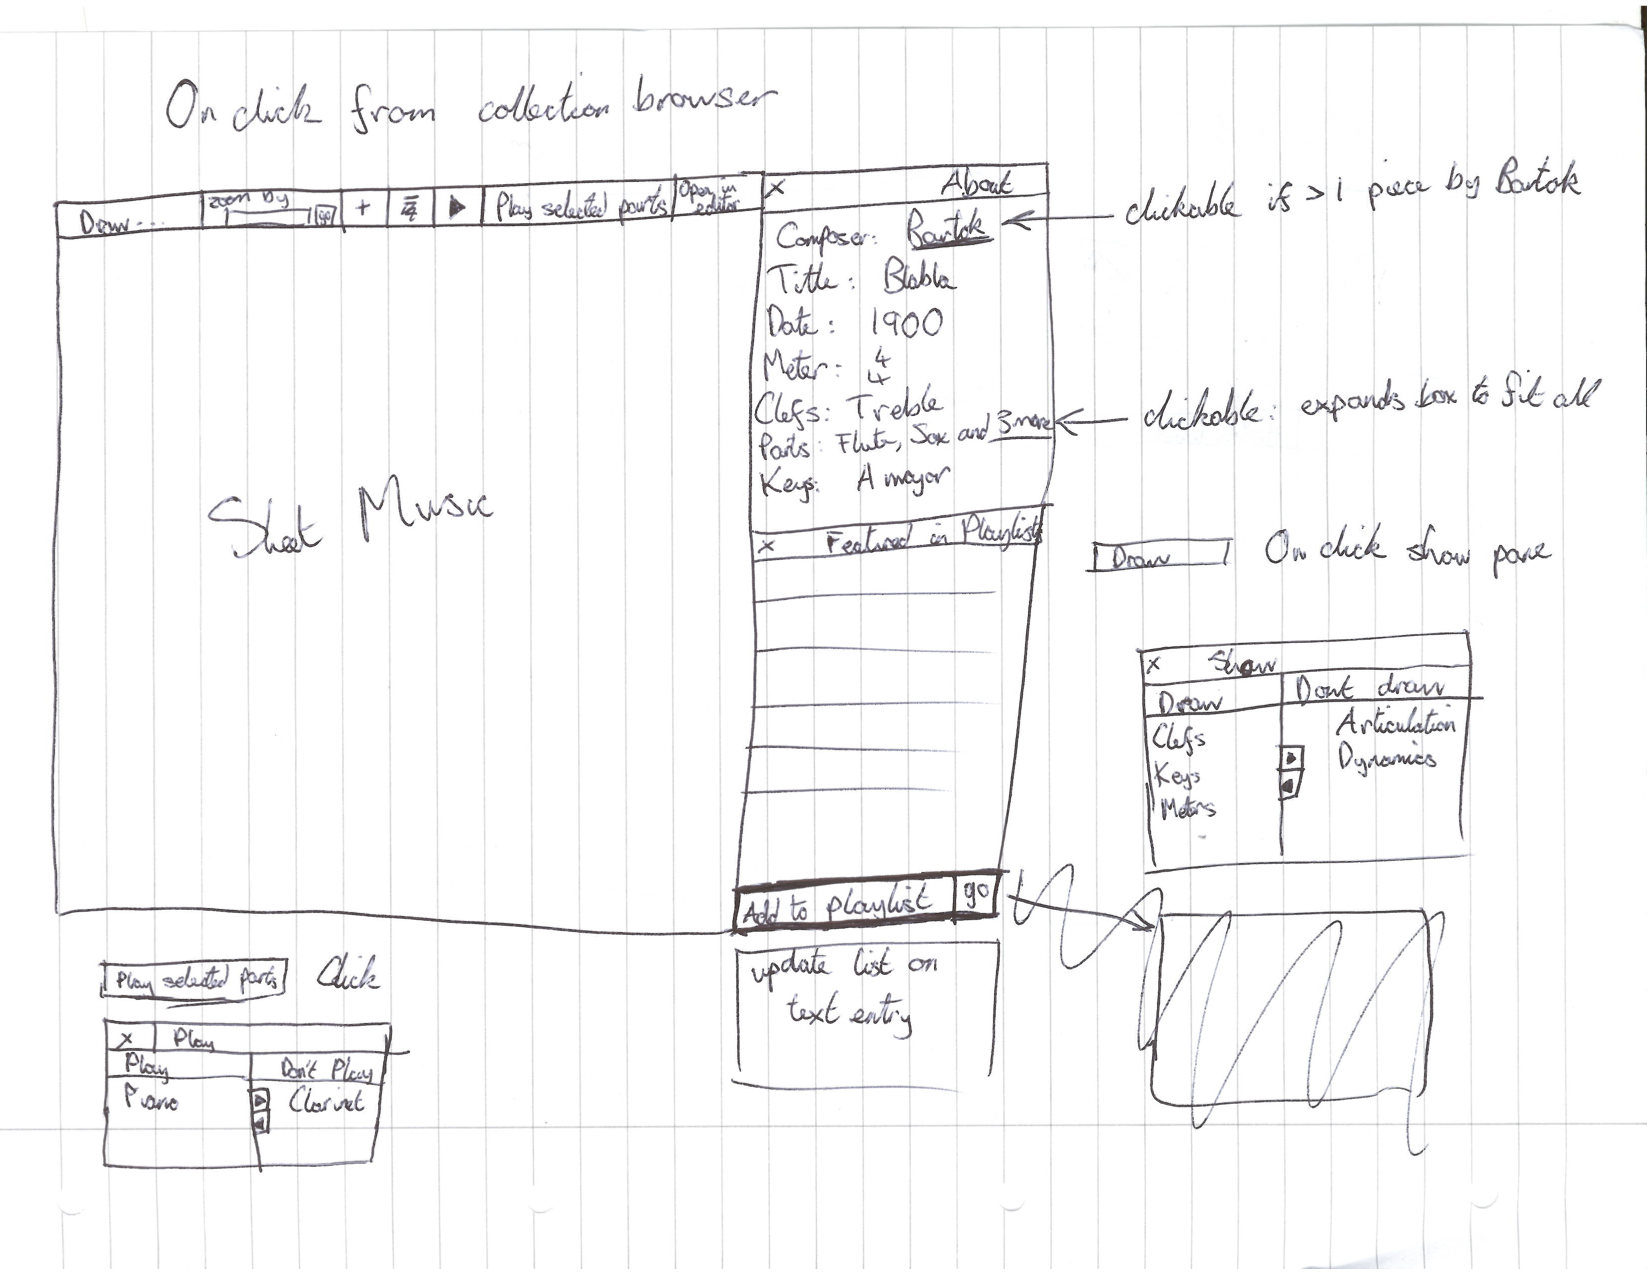
\includegraphics[width=400pt]{sheet_music_view.png}
\subsection{Changes to main display when playlist is selected}
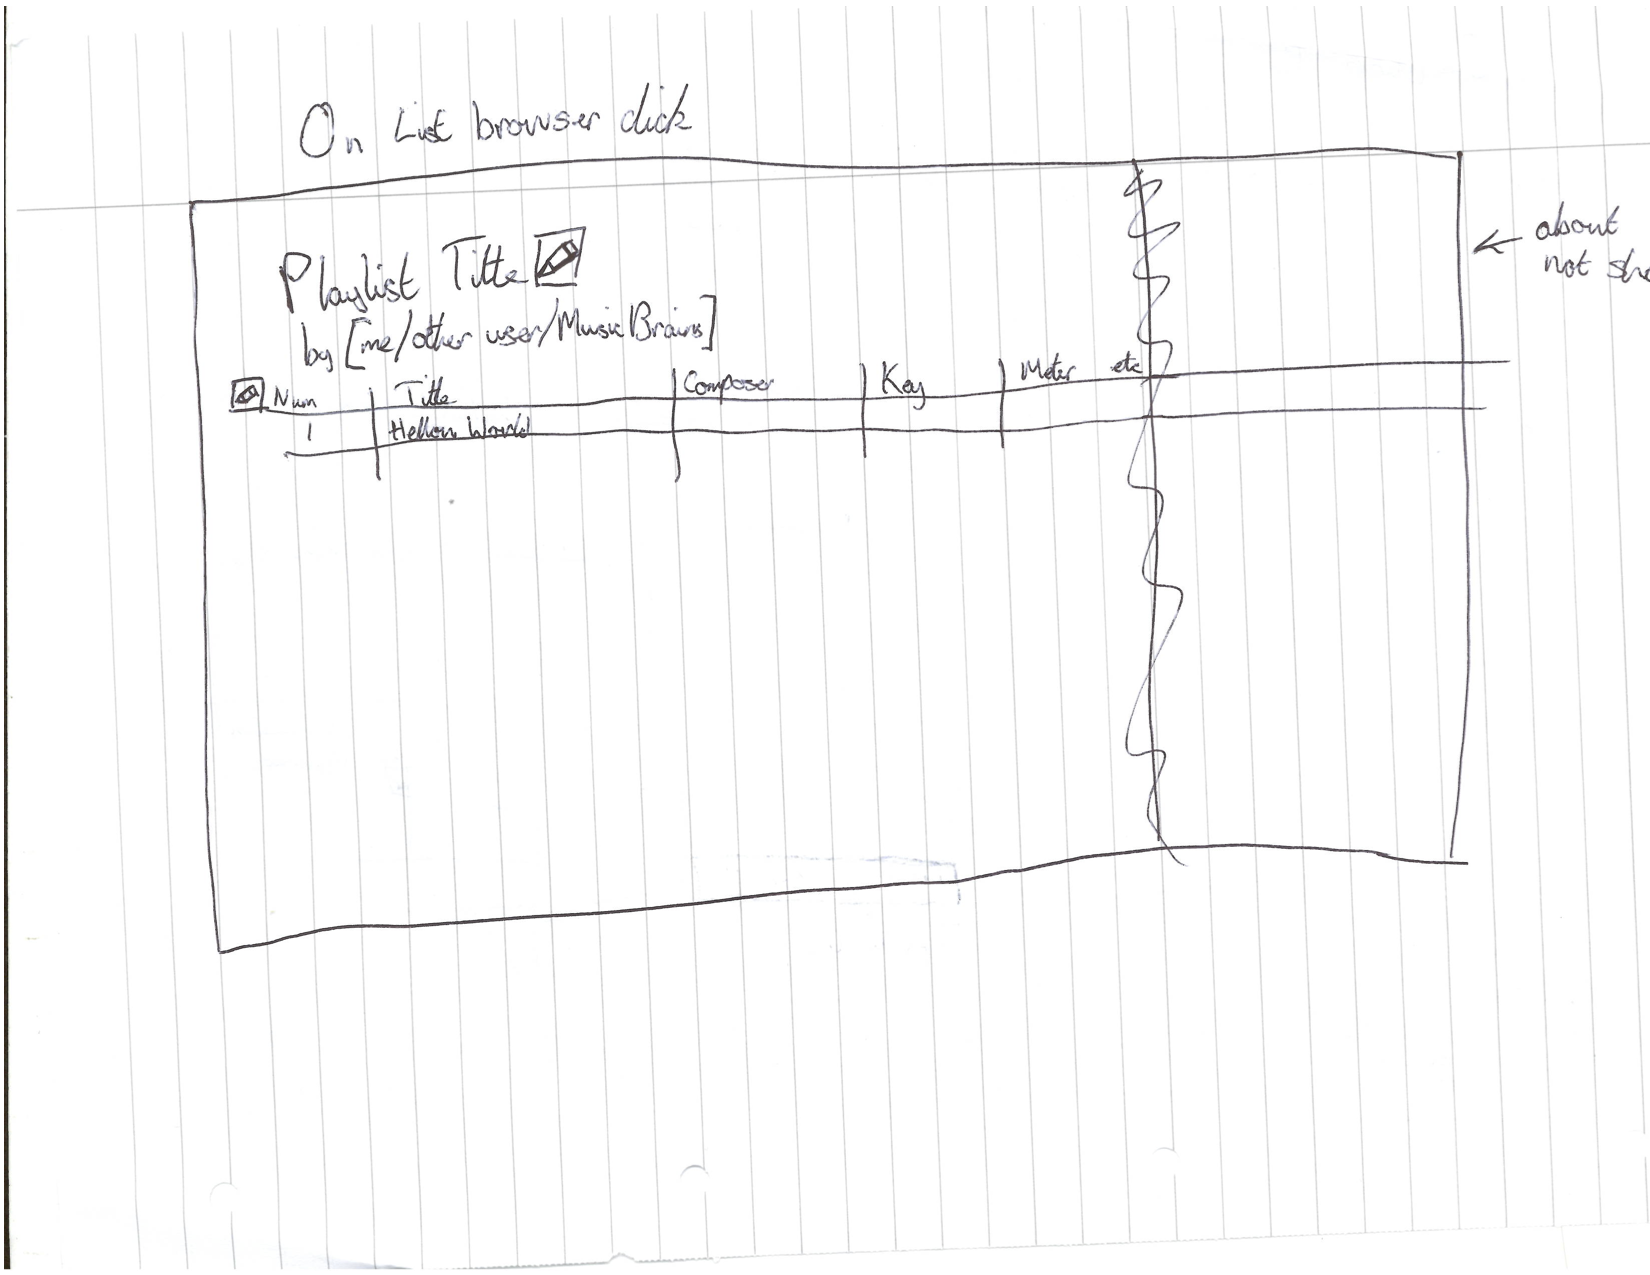
\includegraphics[width=500pt]{playlist_view.png}
\subsection{Other Panes and Popup windows}
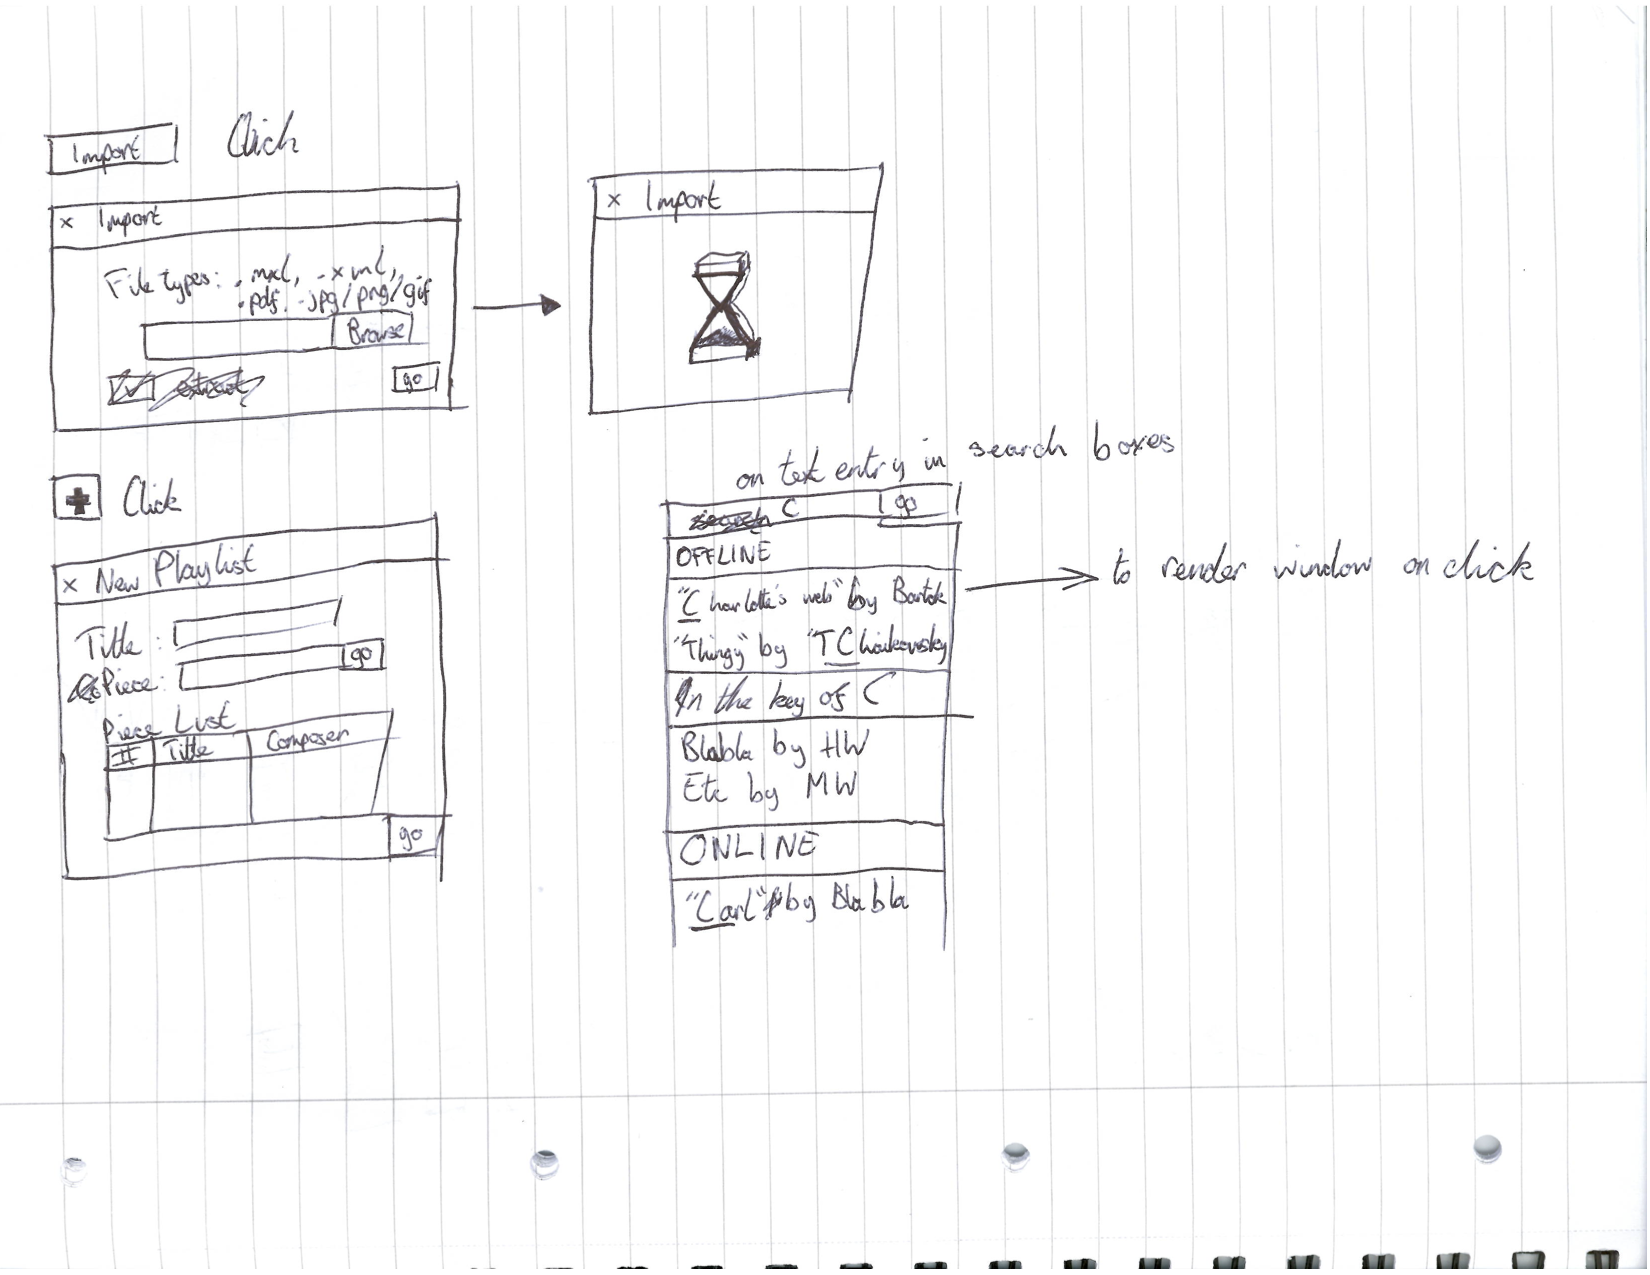
\includegraphics[width=500pt]{other_panes_and_popups}
\end{appendices}

\end{document}
